\documentclass{cuxarticle}
\begin{document}
% タイトル
\begin{titlepage}
  \begin{titlepage}
  \begin{center}
    {\large 2024年度 学士学位論文}\\
    \vspace{19\zh}
    {\Huge 環境情報のセンシングを用いた他者の\\環境評価を表現するロボットシステム}\\ % タイトル
    % {\Large ―サブタイトル―}\\ % サブタイトル(なければコメントアウト)
    \vspace{22\zh}
    \large{
      宮城大学 事業構想学群 価値創造デザイン学類\\
      感性情報デザインコース\\
      \vspace{1\zh}
      22120165\\ % 学籍番号
      中村 龍造\\ % 著者
      \vspace{3\zh}
      指導教員 佐藤 弘樹 准教授
    }
  \end{center}
\end{titlepage}

\end{titlepage}
% アブスト
\begin{center}
  {\Large
    論 文 要 旨\\
    \vspace{2\zh}
    環境情報のセンシングを用いた他者の\\環境評価を表現するロボットシステム\\
    \vspace{2\zh}
  }
\end{center}

%   アブスト本文
本研究では、生活環境における他者の環境評価を表現するロボットシステムを提案する。我々は日常において、人間、動植物、モノなど多様な「他者」と共存している。他者はそれぞれ独自の感覚や基準で環境を評価しているが、我々がそれを直接知ることは難しい。本システムでは、環境センサーで取得したデータを他者基準で評価し、その評価結果をロボットの身体的動作を通じて表現する。「人間―本システム―外界」という関係を採用することで、従来の「人間―外界」という直接的な関係性を再構築し、相互理解の促進を目指す。

実装では、M5StickCによるセンシングとtoioロボットの動作制御を組み合わせ、人間(気温18-28℃)、猫(気温30-38℃)、バナナ(気温14-20℃、湿度45-85\%)、衣服(湿度65\%以下)など異なる他者の環境評価を表現するシステムを実装した。コンポーネント指向アーキテクチャを採用することで、システムの拡張性と保守性を確保し、「弱いロボット」のコンセプトを取り入れた動作表現により、ユーザーに自然な気づきを与えることを目指した。

検証の結果、「よたよた」とした「弱さ」を感じさせる動きの表現や、同一ロボットでの他者の識別性など、いくつかの課題が明らかになった。しかし、本システムは生活環境における多様な他者理解を支援する新たな手法として、人間と他者の相互理解を促進し、多様な存在と相互作用する生活空間の発展に貢献する可能性を示した。さらに介護シーン、遠隔ワーク環境、植物ケアなど具体的なユースケースへの応用可能性についても検討を行った。

\vspace{3\zh}

\begin{flushright}
  宮城大学 事業構想学群 価値創造デザイン学類 感性情報デザインコース\\
  22120165\\ % 学籍番号
  中村 龍造\\ % 著者
\end{flushright}

% 目次
\tableofcontents

\chapter{序論}

\section{研究背景}
我々は生活環境において,人間,動植物,モノなどの多様な「他者」と共存している.他者はそれぞれ独自の感覚や基準で世界を認識しており,我々がそれを直接知ることはできない.近年,脱人間中心デザインの観点から,他者理解の重要性が指摘されている.しかしながら,他者の感覚や基準を共有することは難しく,生活環境において継続的に他者理解を支援する手法は十分に確立されていない.

このような課題に対して,他者の感覚を人間に理解可能な形で表現・仲介するシステムが求められている.特に日常生活の中で自然に他者視点を取り入れる手法は,脱人間中心の実践として重要である.システム化によって他者の感覚を「翻訳」し,それを生活環境内で継続的に提示することで,人間と他者の新たな共生関係を構築できる可能性がある.

同じ人間どうしであっても,個人差によって環境への評価や感覚には違いがある.このような状況において,生活空間に小さな存在が配置され,他者の感覚を代弁することで,私たちの生活をより豊かにする可能性がある.

\section{関連研究}

\subsection{他者視点の表現}
他者視点の表現に関する取り組みとして,次の2つの事例を挙げる.

\subsubsection{In the Eyes of the Animal}
In the Eyes of the Animal\cite{--EyesAnimal}は,動物の環世界(Umwelt)をVRを用いて表現し,環世界を通して森林環境を体験する没入型作品である.ユクスキュルが提唱した「環世界(Umwelt)」の概念に基づき,各生物種が独自の感覚能力と認知特性によって形成する主観的な知覚世界を表現している.

本事例はVR体験に限定されており,実際の生活環境で継続的に他者理解を支援することは困難である.また動物の知覚を一時的な没入体験としてのみ提示しており,長期的な相互作用の可能性については考慮されていない.

\subsubsection{rapotosis}
rapotosis\cite{--ソンヨン}では,衣服を他者として表現している.本事例では,ロボットやwebサービスを用いて,一定期間使用されていない衣服がハンガーから落下するなどといった体験を通して,衣服が自律的に「自殺」するプロセスを表現している.具体的な実装としては,ハンガーから服が自動的に落下する装置や,衣服がSNSを通してユーザにメッセージを送信する機能.所有者の同意を得た後に自動的に出品される仕組みや,新しい所有者が決まると自走するダンボールで回収されるシステムから構成される.

本事例では特定の衣服という限定的な対象にのみ表現対象として焦点を当てており,より広範な他者の感覚表現には至っていない.

\subsection{環境センシング}
環境センシングシステムでは,個々人基準の環境評価の重要性が示されている\cite{Saini-2020-IndoorAirQualityMonitoring}.環境センシングシステムは,湿度,CO2,CO,PM2.5,VOCsなどの環境パラメータを測定し,居住環境の質を継続的に監視する.しかし,これらの情報はアプリケーションの視覚的UIを通じて一方的に表示されることが多く,利用者とシステム間の双方向的なインタラクションや,身体的動作による環境情報の表現と理解を促す事例は限られている.また,多くの既存システムは実験室や管理された環境で評価されており,実際のフィールド環境におけるIAQパラメータの信頼性の高い意思決定,評価,測定に課題が残る.

\subsection{HRIの先行事例}
本研究に関連するロボットインタラクションの先行事例として,次の2例を挙げる.

\subsubsection{HERMITS}
HERMITS\cite{--HERMITSProceedings33rdAnnual}は,1つの自走式ロボットに対して「シェル」と呼ばれる外装を切り替えることで,異なる機能の提供を可能とする試みである.これらのシェルはロボットの移動能力を利用して動的に再構成される.HERMITSのアプローチはシンプルなロボットを用いて,多様な相互作用機能をもたらす新しいTUIの可能性を示している.

本研究では,この考え方をソフトウェア的に実装し,同一のロボットハードウェアで多様な他者を表現することを目指した.

\subsubsection{弱いロボット}
岡田らの提案する「弱いロボット」\cite{岡田-2017-弱いロボ}は,あえて「弱さ」を表現する動作をデザインすることで,人間を積極的にタスク遂行に取り入れるロボットである.ロボットの完全性や自律性を追求するのではなく,むしろ「不完全さ」や「弱さ」を意図的にデザインに取り入れることで,人間との関係性を強化することを狙っている.例えば,「ゴミ箱ロボット」\cite{岡田美智男-2012-ゴミ箱ロ}は一人ではゴミを拾えないが,子どもたちのアシストを引き出すことで結果的にゴミを収集できる.また「Talking-Ally」\cite{岡田美智男-2012-ゴミ箱ロ}は会話の中で言い淀みや言い直しを活用し,聞き手と相互に会話の調整を行う.これらのロボットは「個体」としての能力を抑制しながらも,周囲との「関係」を通じて豊かな相互作用を生み出している.本研究では,この「弱さ」の表現を取り入れ,自然な形で人間の注意を効果的に喚起する手法を検討した.

\section{研究目的}
関連研究を踏まえ本研究では,生活空間における他者の環境評価を,身体的動作によって表現するロボットシステムを提案する.センサーで取得した環境データを他者基準で評価し,その評価結果をロボットの身体的動作を通じて表現する.生活空間にロボットを分散配置することで,継続的な他者表現を可能とする.また,他者の表現手段を身体的動作とすることで,同一のロボットで多様な他者表現を可能とすることを目指す.

図\ref{fig:system-concept}のような,身の回りで他者の感覚を代弁する小型ロボットが活動するシステムを実装することで,人間と他者の相互理解を促進し,多様な存在が共存する生活空間の実現に貢献する.

\begin{figure}[h]
  \centering
  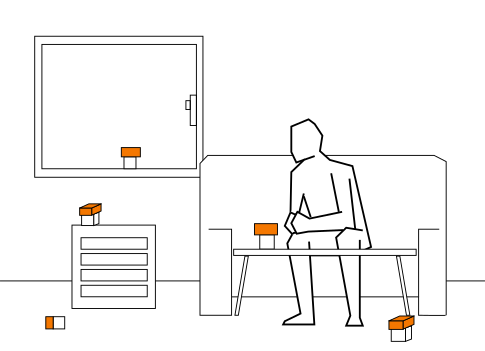
\includegraphics[keepaspectratio,height=0.2\textheight]{resources/robot-in-house.png}
  \caption[short]{本システムの構想図.\\生活空間に分散配置された小型ロボットが他者の感覚を代弁する.}
  \label{fig:system-concept}
\end{figure}

\chapter{提案システム}

\section{システム要件}
研究目的を踏まえ,本システムの要件として以下の3点を設定した

\begin{enumerate}
  \item 生活環境で継続的に他者の環境評価を表現できる
  \item 多様な他者を表現できる
  \item 特別な操作なしでの自然な他者理解を支援できる
\end{enumerate}

\section{システム構成}
本システムの構成について,システム全体のフロー,ハードウェア構成,ソフトウェア構成の3点を述べる.

\subsection{システム全体のフロー}
システムの全体のフローは,以下の4つのフェーズから構成される.

\begin{enumerate}
  \item \textbf{センシングフェーズ}:センサーが環境データを取得し,ロボットシステムに送信する
  \item \textbf{評価フェーズ}:受信した環境データを他者個別の基準で評価し,環境に対する評価結果を出力する
  \item \textbf{アクション決定フェーズ}:評価結果に基づき,他者の環境評価を表現するアクションを決定する
  \item \textbf{実行フェーズ}:決定されたアクションをロボットに送信し,実行する
\end{enumerate}

このサイクルは継続的に実行され,環境の変化に応じてリアルタイムに他者の環境評価が表現される仕組みとなっている.システム全体のフロー図を図\ref{fig:system-flow}に示す.

\begin{figure}[h]
  \centering
  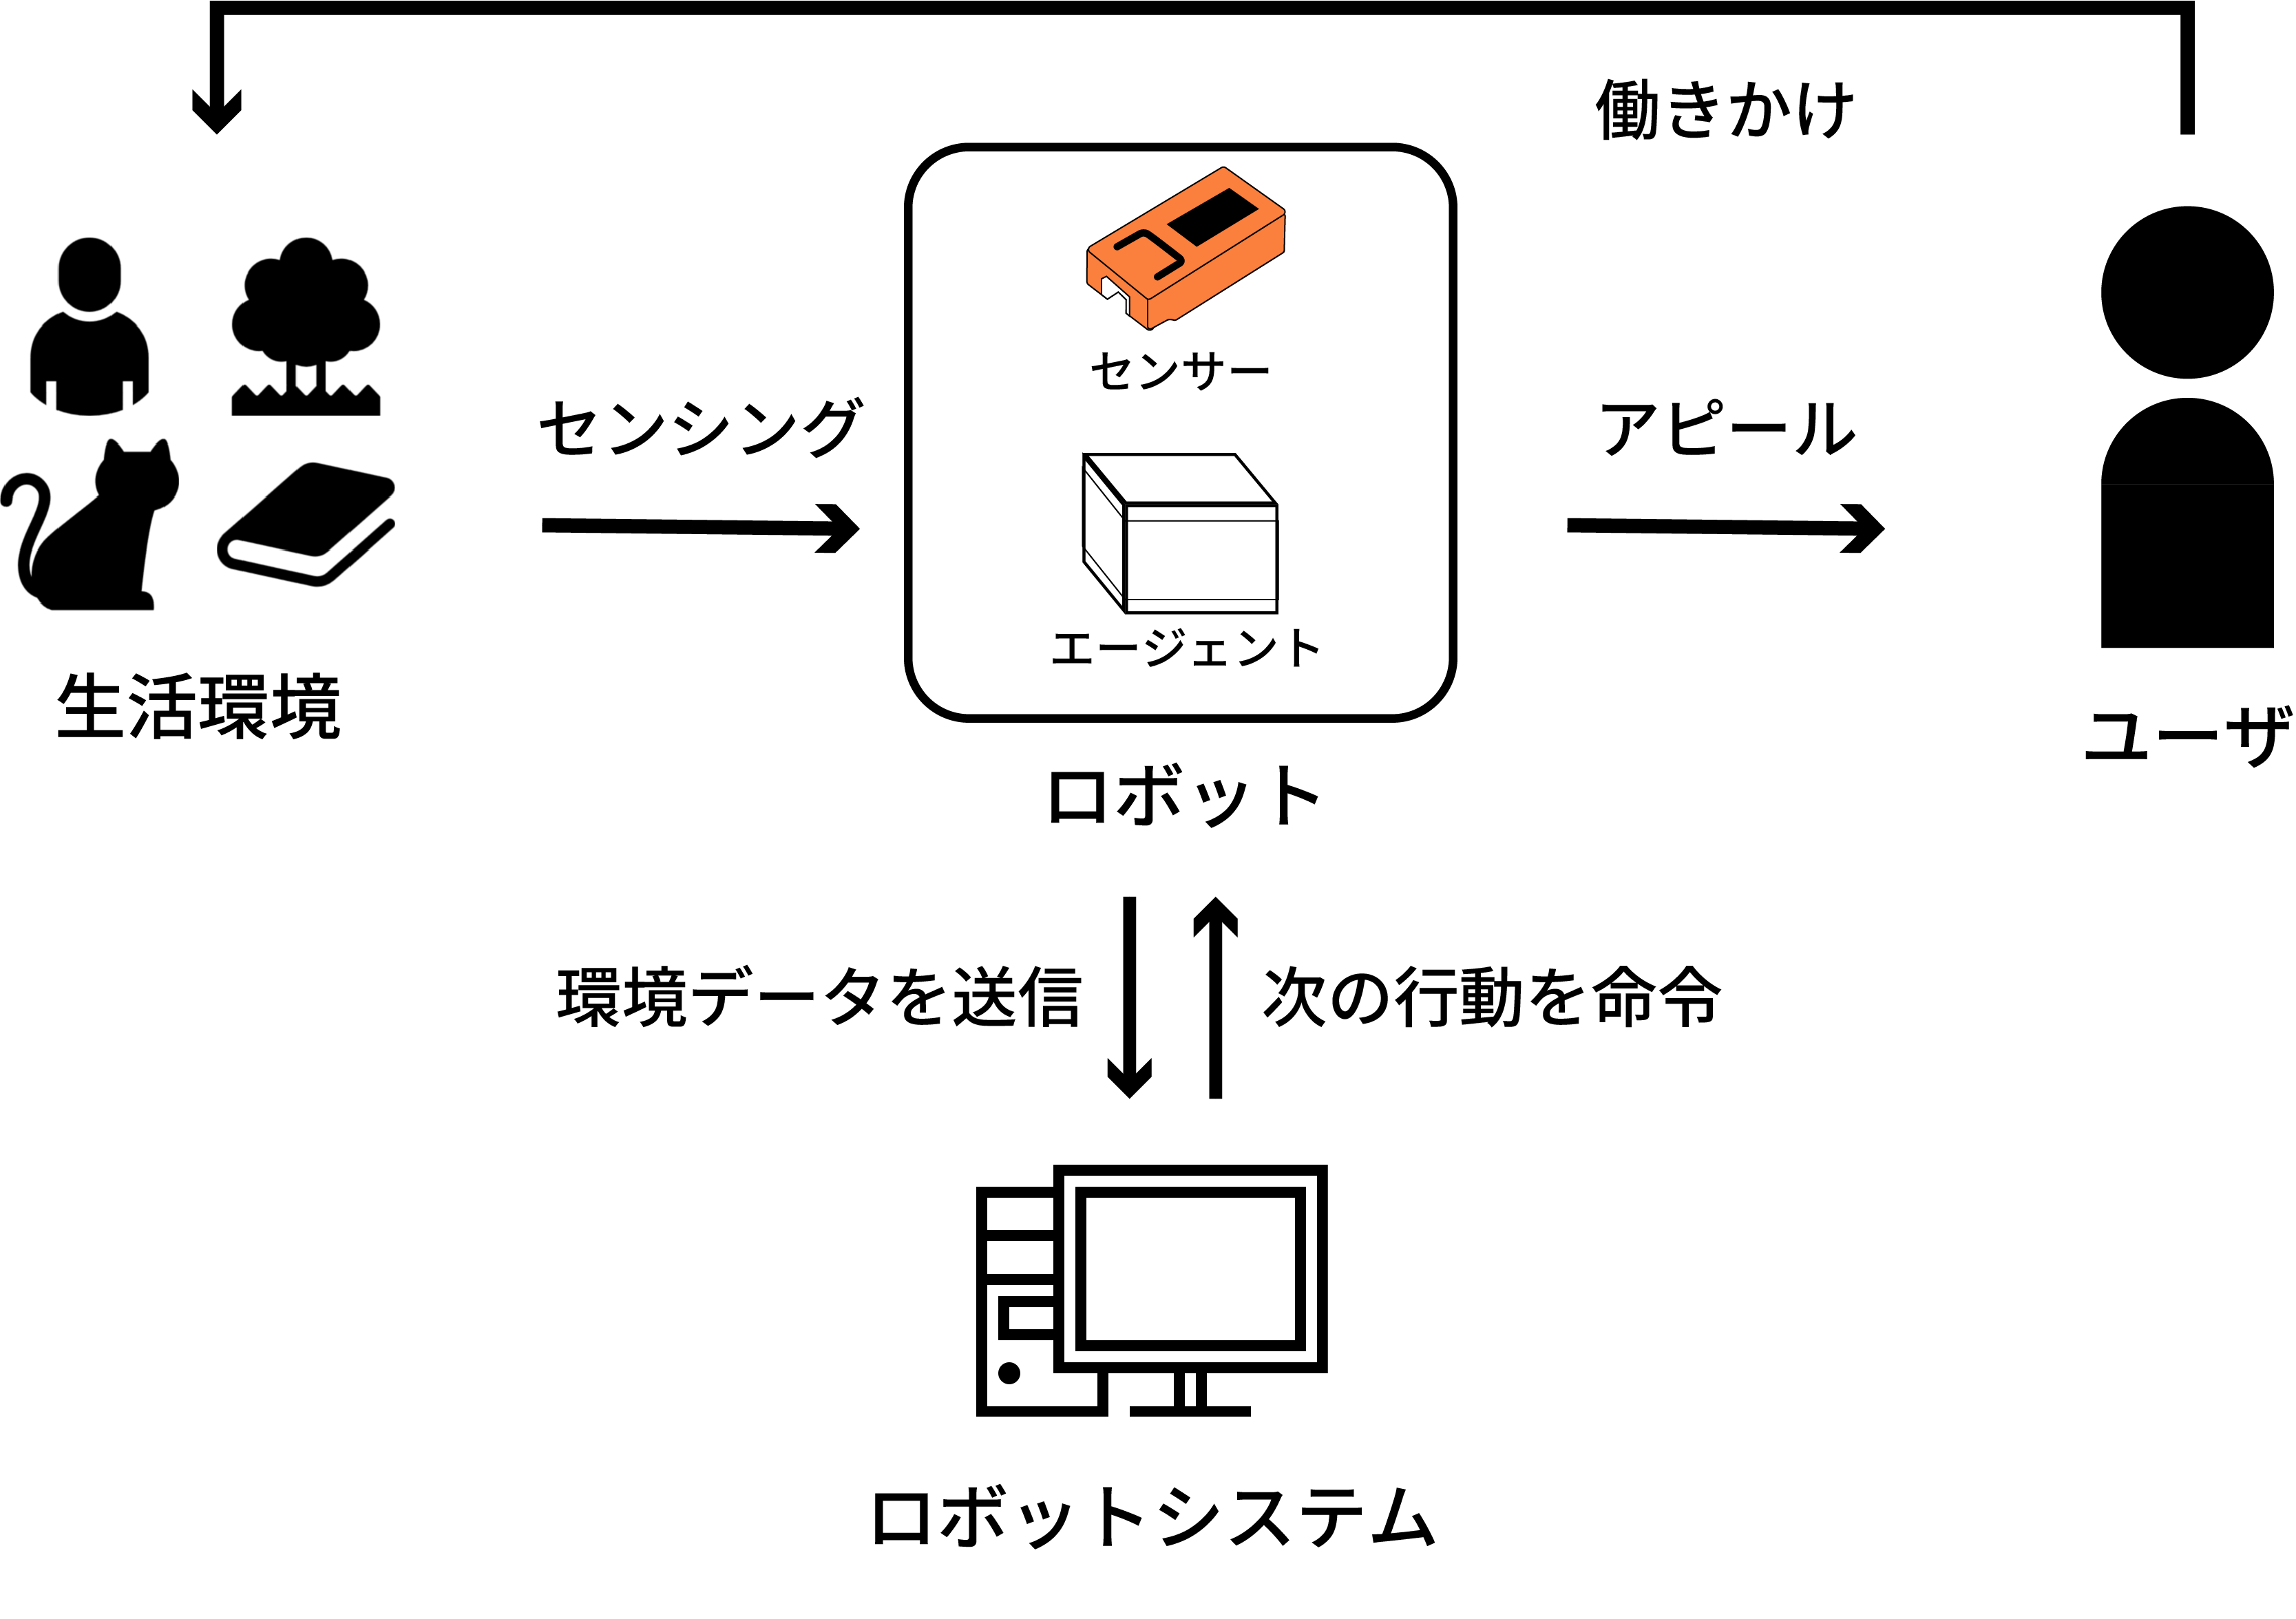
\includegraphics[keepaspectratio, height=0.3\textheight]{resources/system-flow.png}
  \caption[short]{システム全体のフロー図.センシングフェーズ,評価フェーズ,アクション決定フェーズ,実行フェーズの4つのフェーズから構成される.}
  \label{fig:system-flow}
\end{figure}

\subsection{ハードウェア構成}
本システムのハードウェアは,センシングユニットおよびエージェントロボットから構成される.センシングユニットは環境データの取得およびロボットシステムへの送信を行い,エージェントロボットはアクション決定フェーズで決定されたアクションを実行する.

\subsubsection{センシングユニット(M5StickC)}
本研究ではセンシングユニットとして M5StickC(M5Stack社)\cite{--M5StickC}を使用した.選定の主な理由は以下の技術的要因に基づく.

\begin{itemize}
  \item \textbf{スタンドアロン性能}:独立したマイクロコントローラとして機能し,外部PCなどに依存せずに長時間のセンシングが可能
  \item \textbf{高い拡張性}:複数のセンサーモジュールが使用可能であり,多様な環境データを対象としうる
  \item \textbf{コンパクトな形状}:小型・軽量であり,生活空間内の様々な場所に設置可能なほか,エージェントロボットへの積載が可能
  \item \textbf{無線通信}:Wi-Fi,Bluetoothなどの無線通信機能を内蔵し,システム内のデータ連携が容易
  \item \textbf{開発環境}:Arduino IDEやPlatformIOを用いた標準的な開発環境が整備されている
\end{itemize}

\subsubsection{エージェントロボット(toio)}
エージェントロボットにはtoio(SONY社)\cite{--小さなキ}を使用した.理由は次の技術的要件を満たしていたためである.

\begin{itemize}
  \item \textbf{マルチモーダルな表現能力}:移動,LEDによる色表現,音声出力など,複数のモダリティによる表現が可能
  \item \textbf{スケーラビリティ}:複数台を同時制御するスワームロボットとしての利用が可能
  \item \textbf{豊富な開発環境}:Unity,JavaScript,Pythonなど複数の開発言語やフレームワークとの互換性が高い
  \item \textbf{先行研究の存在}:HERMITS\cite{--HERMITSProceedings33rdAnnual}のような先行研究が存在する.
\end{itemize}

\subsection{ソフトウェア構成}
ソフトウェア部分の構成図を図\ref{fig:software-architecture}に示す.
\begin{figure}[h]
  \centering
  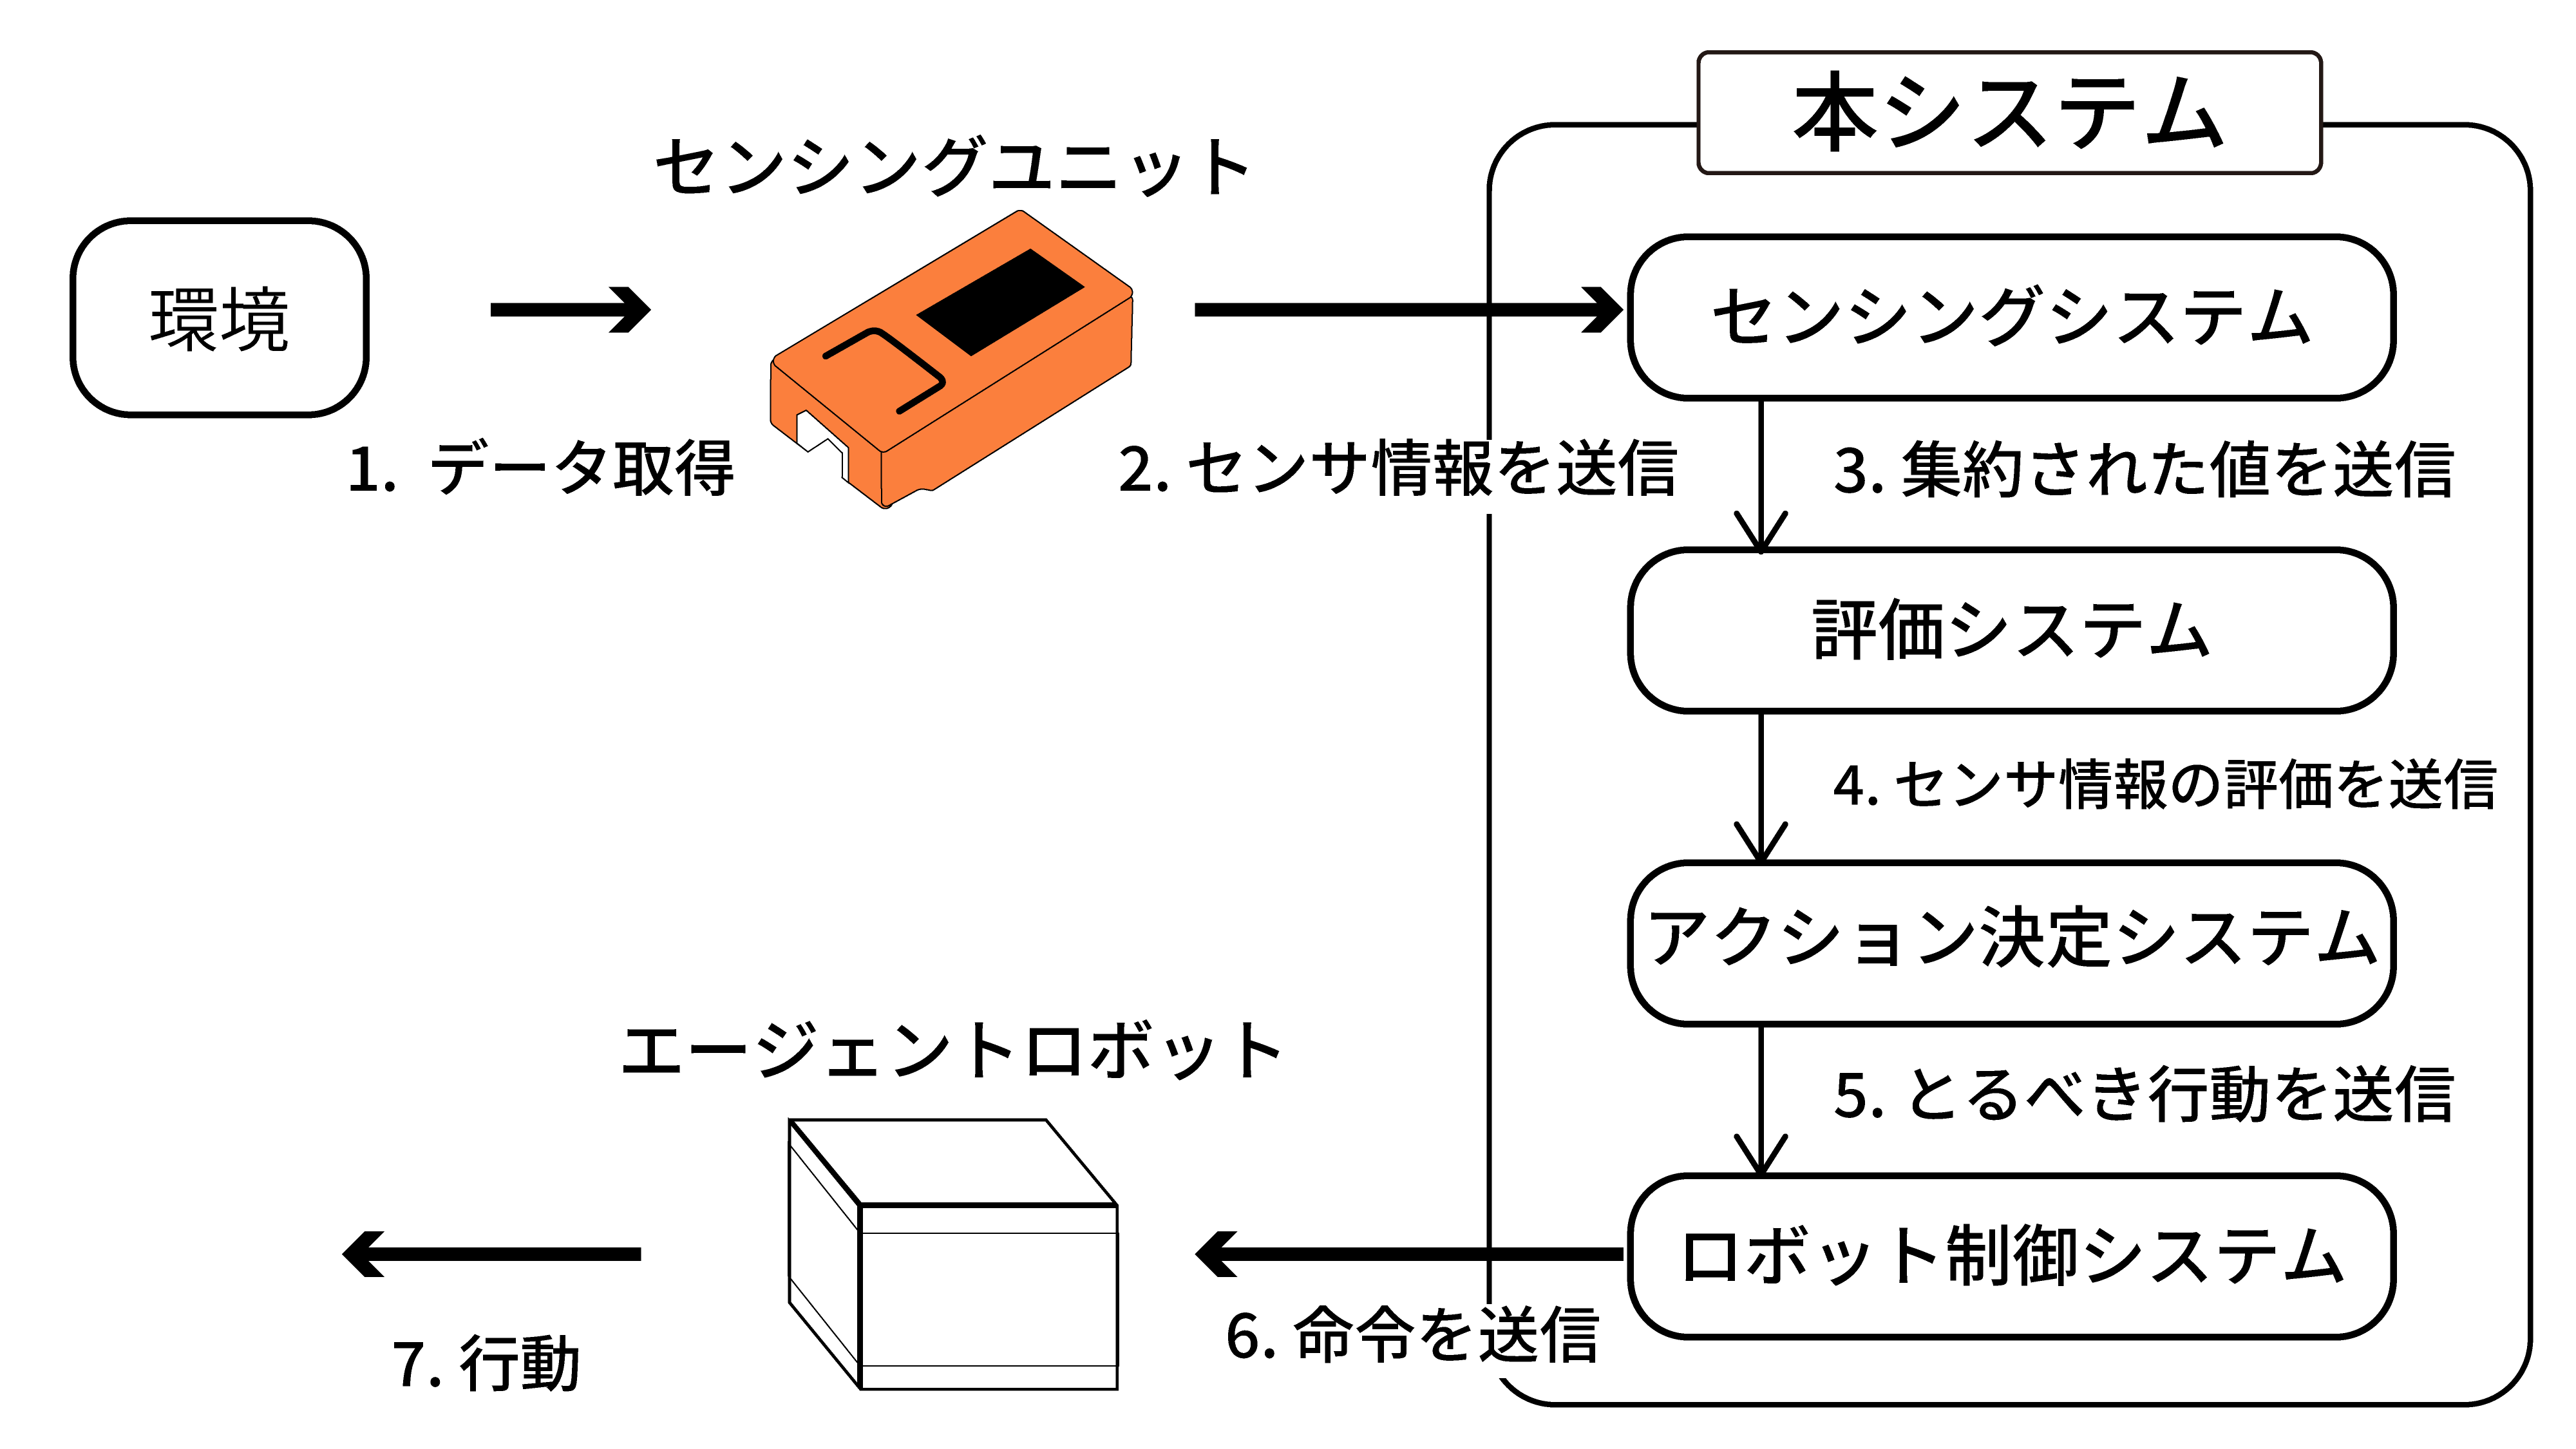
\includegraphics[keepaspectratio, width=0.6\columnwidth]{resources/system_structure.png}
  \caption[short]{}
  \label{fig:software-architecture}
\end{figure}

本システムのソフトウェアは,Unity環境で実装され,以下の4つの主要コンポーネントから構成される.

\begin{enumerate}
  \item センシングシステム:環境データの取得と処理
  \item 評価システム:他者基準での環境データの評価
  \item アクション決定システム:評価結果に基づく動作の決定
  \item ロボット制御システム:決定された動作の実行
\end{enumerate}

以下,各コンポーネントの詳細について説明する.

\subsubsection{センシングシステム}
センシングシステムは,センシングユニットからのデータ取得とその処理を担当する.

センシングユニットで取得された環境データはBluetooth通信でセンシングシステムに送信され,デシリアライズされる.センシングシステムは受信データを構造化し,他のコンポーネントに渡す.環境データごとにセンサーインタフェースを抽象化することで,新しいセンサーの追加が容易なほか,異なるセンサーであっても,同じインタフェースを介してデータの取得が可能である.

センシングユニット側のプログラムはPlatformIOを用いて開発した.

\subsubsection{評価システム}
評価システムは,センシングシステムから受け取った環境データを他者固有の基準で評価し,結果を生成する.

評価システムでは予め定義された他者の基準値と環境データとの差分を計算し,評価結果を生成する.評価結果はスコアとして表現され,他者の環境評価を表す.基準値はUnityエディタ上で設定可能であり,他者ごとに異なる基準値を設定することができる.複数の環境データを評価する場合,基準値からの差分では評価値の重要度が均等になるため,各評価値に重みを設定し,総合評価スコアとして算出している.なおこれらの評価ロジックは開発者側で定義するため,他者の基準値や評価ロジックを柔軟に変更することが可能である.

例えば猫の適温評価では,猫にとっての快適温度(30~38℃)を基準とし,スコアは現在の温度がこの範囲を下回ると負に,上回ると正に増加する.スコアはアクション決定システムによって,動作の種類や強度の決定に使用される.

評価システムは他者とそれが評価する環境データのパターンごとに,個別の実装が必要である.

\subsubsection{アクション決定システム}
アクション決定システムは,評価システムから受け取ったスコアに基づいて,他者の状態を表現するための適切なアクションを決定する.

アクション決定システムは他者のパターンごとに実装されたアクションデータを参照し,スコアに応じたアクションを選択する.アクションデータは,モーター制御命令のキュー,音声出力命令のキュー,LED制御命令のキュー,次の動作命令までの時間,アクション全体の完了に必要な時間などの要素を含むAction構造体として管理される.アクションデータはActionLibraryによって管理され,再利用可能なアクションパターンを提供する.

アクション決定システムも評価システム同様,他者および対象となる環境データごとに異なるアクションパターンを実装する必要がある.

\subsubsection{ロボット制御システム}
ロボット制御システムは,アクション決定システムから受け取ったアクション命令をtoioに適切に送信し,実行を管理する.

toioにはUnityでの開発をサポートするtoio SDKライブラリが提供されており,本システムではこのライブラリを用いてtoioの制御を行っている.ロボット制御システムはtoio SDKライブラリをラップし,動作に必要なクラスや関数を提供する.

アクション決定システムで生成されたアクションデータは,ロボット制御システムによってtoioに送信され,実行される.アクションはキューとして処理され,現在のアクションが完了されると次のアクションが実行される.またtoio自体にも加速度センサやジャイロセンサ,衝突検知機能が搭載されており,本システムでは衝突検知によって,toioが障害物に衝突した場合の挙動を制御している.

\chapter{実装と評価}

\section{実装した主体と環境データの組み合わせ}
本システムは,人間や動植物,モノなどといった多様な他者を表現可能とすることを目指す.本システムが表現可能な他者の範囲を示すため,本研究では,4種の他者と環境データの組み合わせを実装した.表\ref{table:entities}に実装したパターンの概要を示す.

\begin{table}[htbp]
  \caption{実装した他者-環境データの対応表}
  \label{table:entities}
  \centering
  \begin{tabular}{|l|l|l|}
    \hline
    他者 & 環境データ & アクション \\
    \hline
    人間 & 気温 &  快適時は周囲を歩き回り,不快時は暑がる,寒がるような動作を行う \\
    \hline
    動物(猫) & 気温 & 快適時は香座座りするようにじっとする.不快時は激しく動く \\
    \hline
    食品(バナナ) & 気温,湿度 & 快適時は穏やかに動き,不快時はノロノロと動いて腐敗を表現 \\
    \hline
    衣服 & 湿度 & クローゼット内でユーザの注意を引く \\
    \hline
  \end{tabular}
\end{table}

以下,各パターンの詳細について説明する.

\subsection{人間}
\begin{itemize}
  \item 評価対象:気温(18-28℃)\cite{JianZhuWuHuanJingWeiShengGuanLiJiZhunnituite|HouShengLaoDongSheng}
  \item 動作パターン:
    \begin{itemize}
      \item 快適時:周囲を歩き回る
      \item 不快時(暑い):激しい動作
      \item 不快時(寒い):身体を震わせる
    \end{itemize}
\end{itemize}

\subsection{猫}
\begin{itemize}
  \item 評価対象:気温(30-38℃)\cite{stellaEnvironmentalAspectsDomestic2016}
  \item 動作パターン:
    \begin{itemize}
      \item 快適時:何もしない
      \item 不快時(暑い):激しい動作
      \item 不快時(寒い):身体を震わせる
    \end{itemize}
\end{itemize}

\subsection{バナナ}
\begin{itemize}
  \item 評価対象:
    \begin{itemize}
      \item 気温:14-20℃
      \item 相対湿度:45-85\%\cite{--バナナの}
    \end{itemize}
  \item 動作パターン:3段階の状態表現
    \begin{itemize}
      \item 快適時:黄色のLEDを点灯しながら前進する
      \item 要注意時:音と橙色のLEDを点灯させながら前進する
      \item 警戒時:音声と赤色のLEDを点灯させながら回転する
    \end{itemize}
\end{itemize}

\subsection{衣服}
\begin{itemize}
  \item 評価対象:相対湿度(65\%以下)\cite{--クローゼ}
  \item 動作パターン:
    \begin{itemize}
      \item 快適時:前進して2回転
      \item 要注意時:向きを変えながら前進
      \item 警戒時:不規則に動きながら音とLEDを点灯
    \end{itemize}
\end{itemize}

\section{課題と考察}
本システムの実装後,自己評価および卒業展示での来場者からのフィードバックを得た.図\ref{fig:system-test}に示すように,各他者のパターンを実装し動作確認を行い,以下のような課題が明らかになった:

\begin{figure}[h]
  \centering
  \begin{tabular}{cccc}
    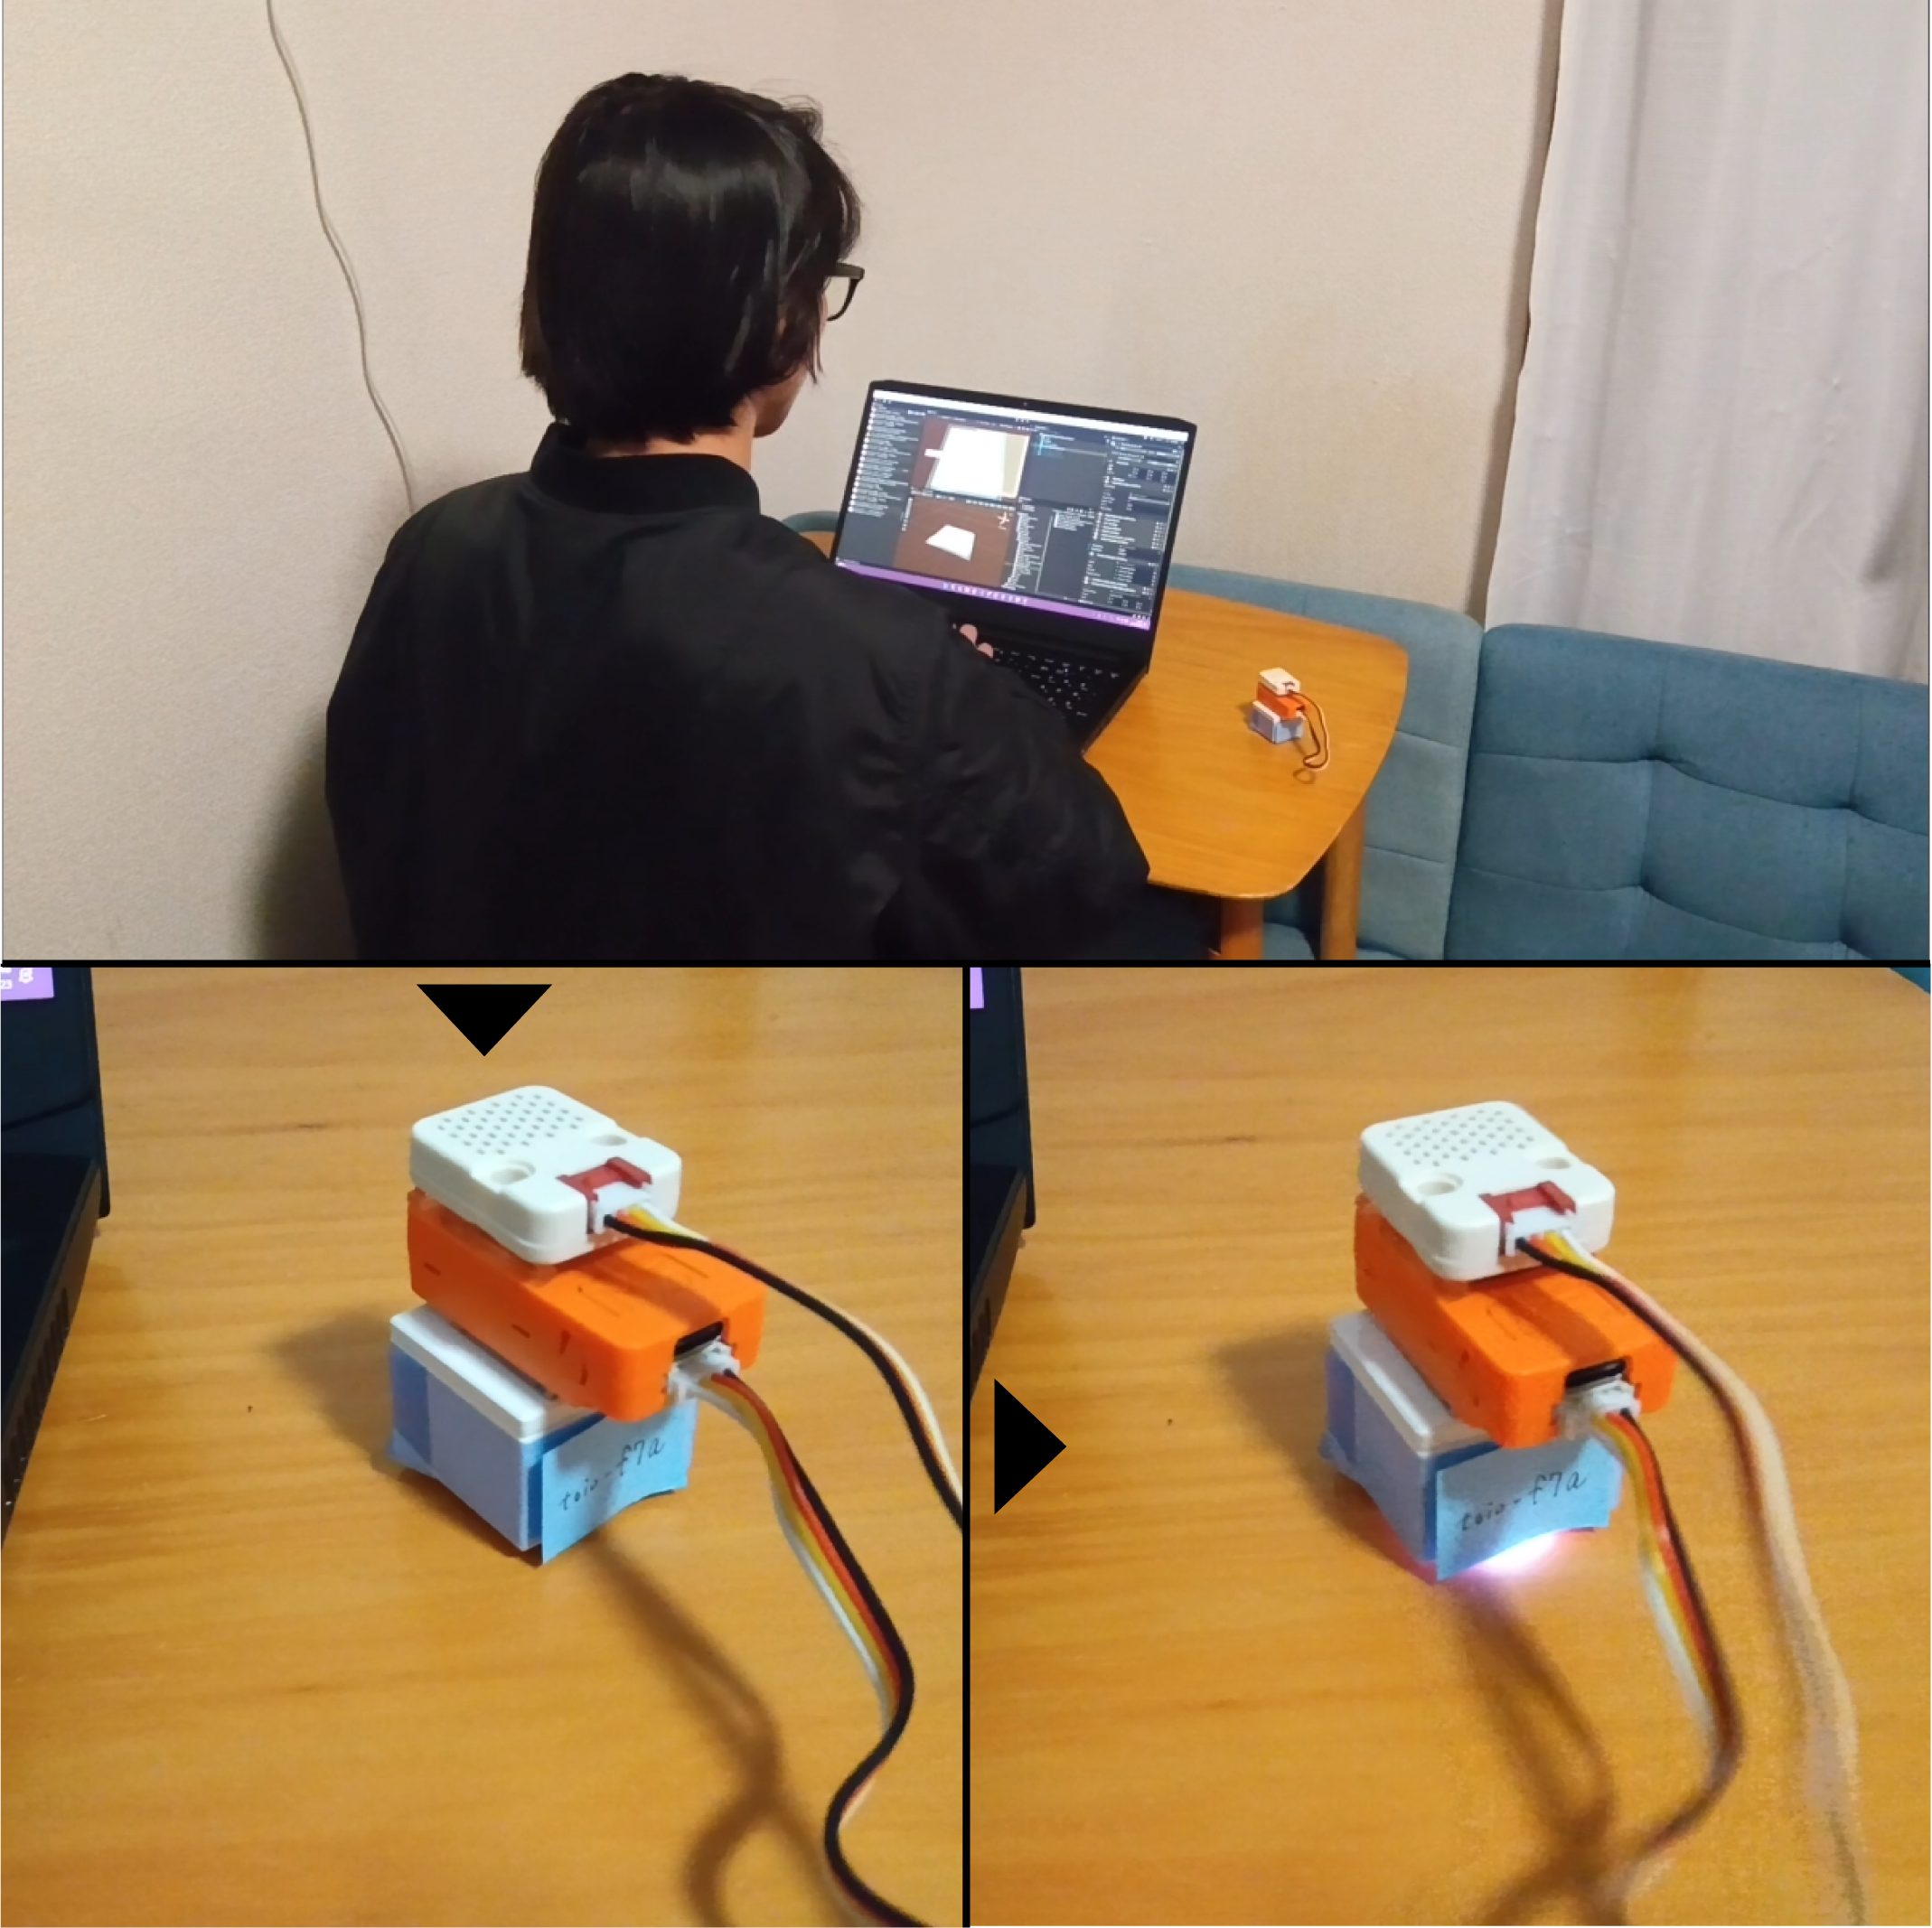
\includegraphics[width=0.22\textwidth]{resources/human.png} &
    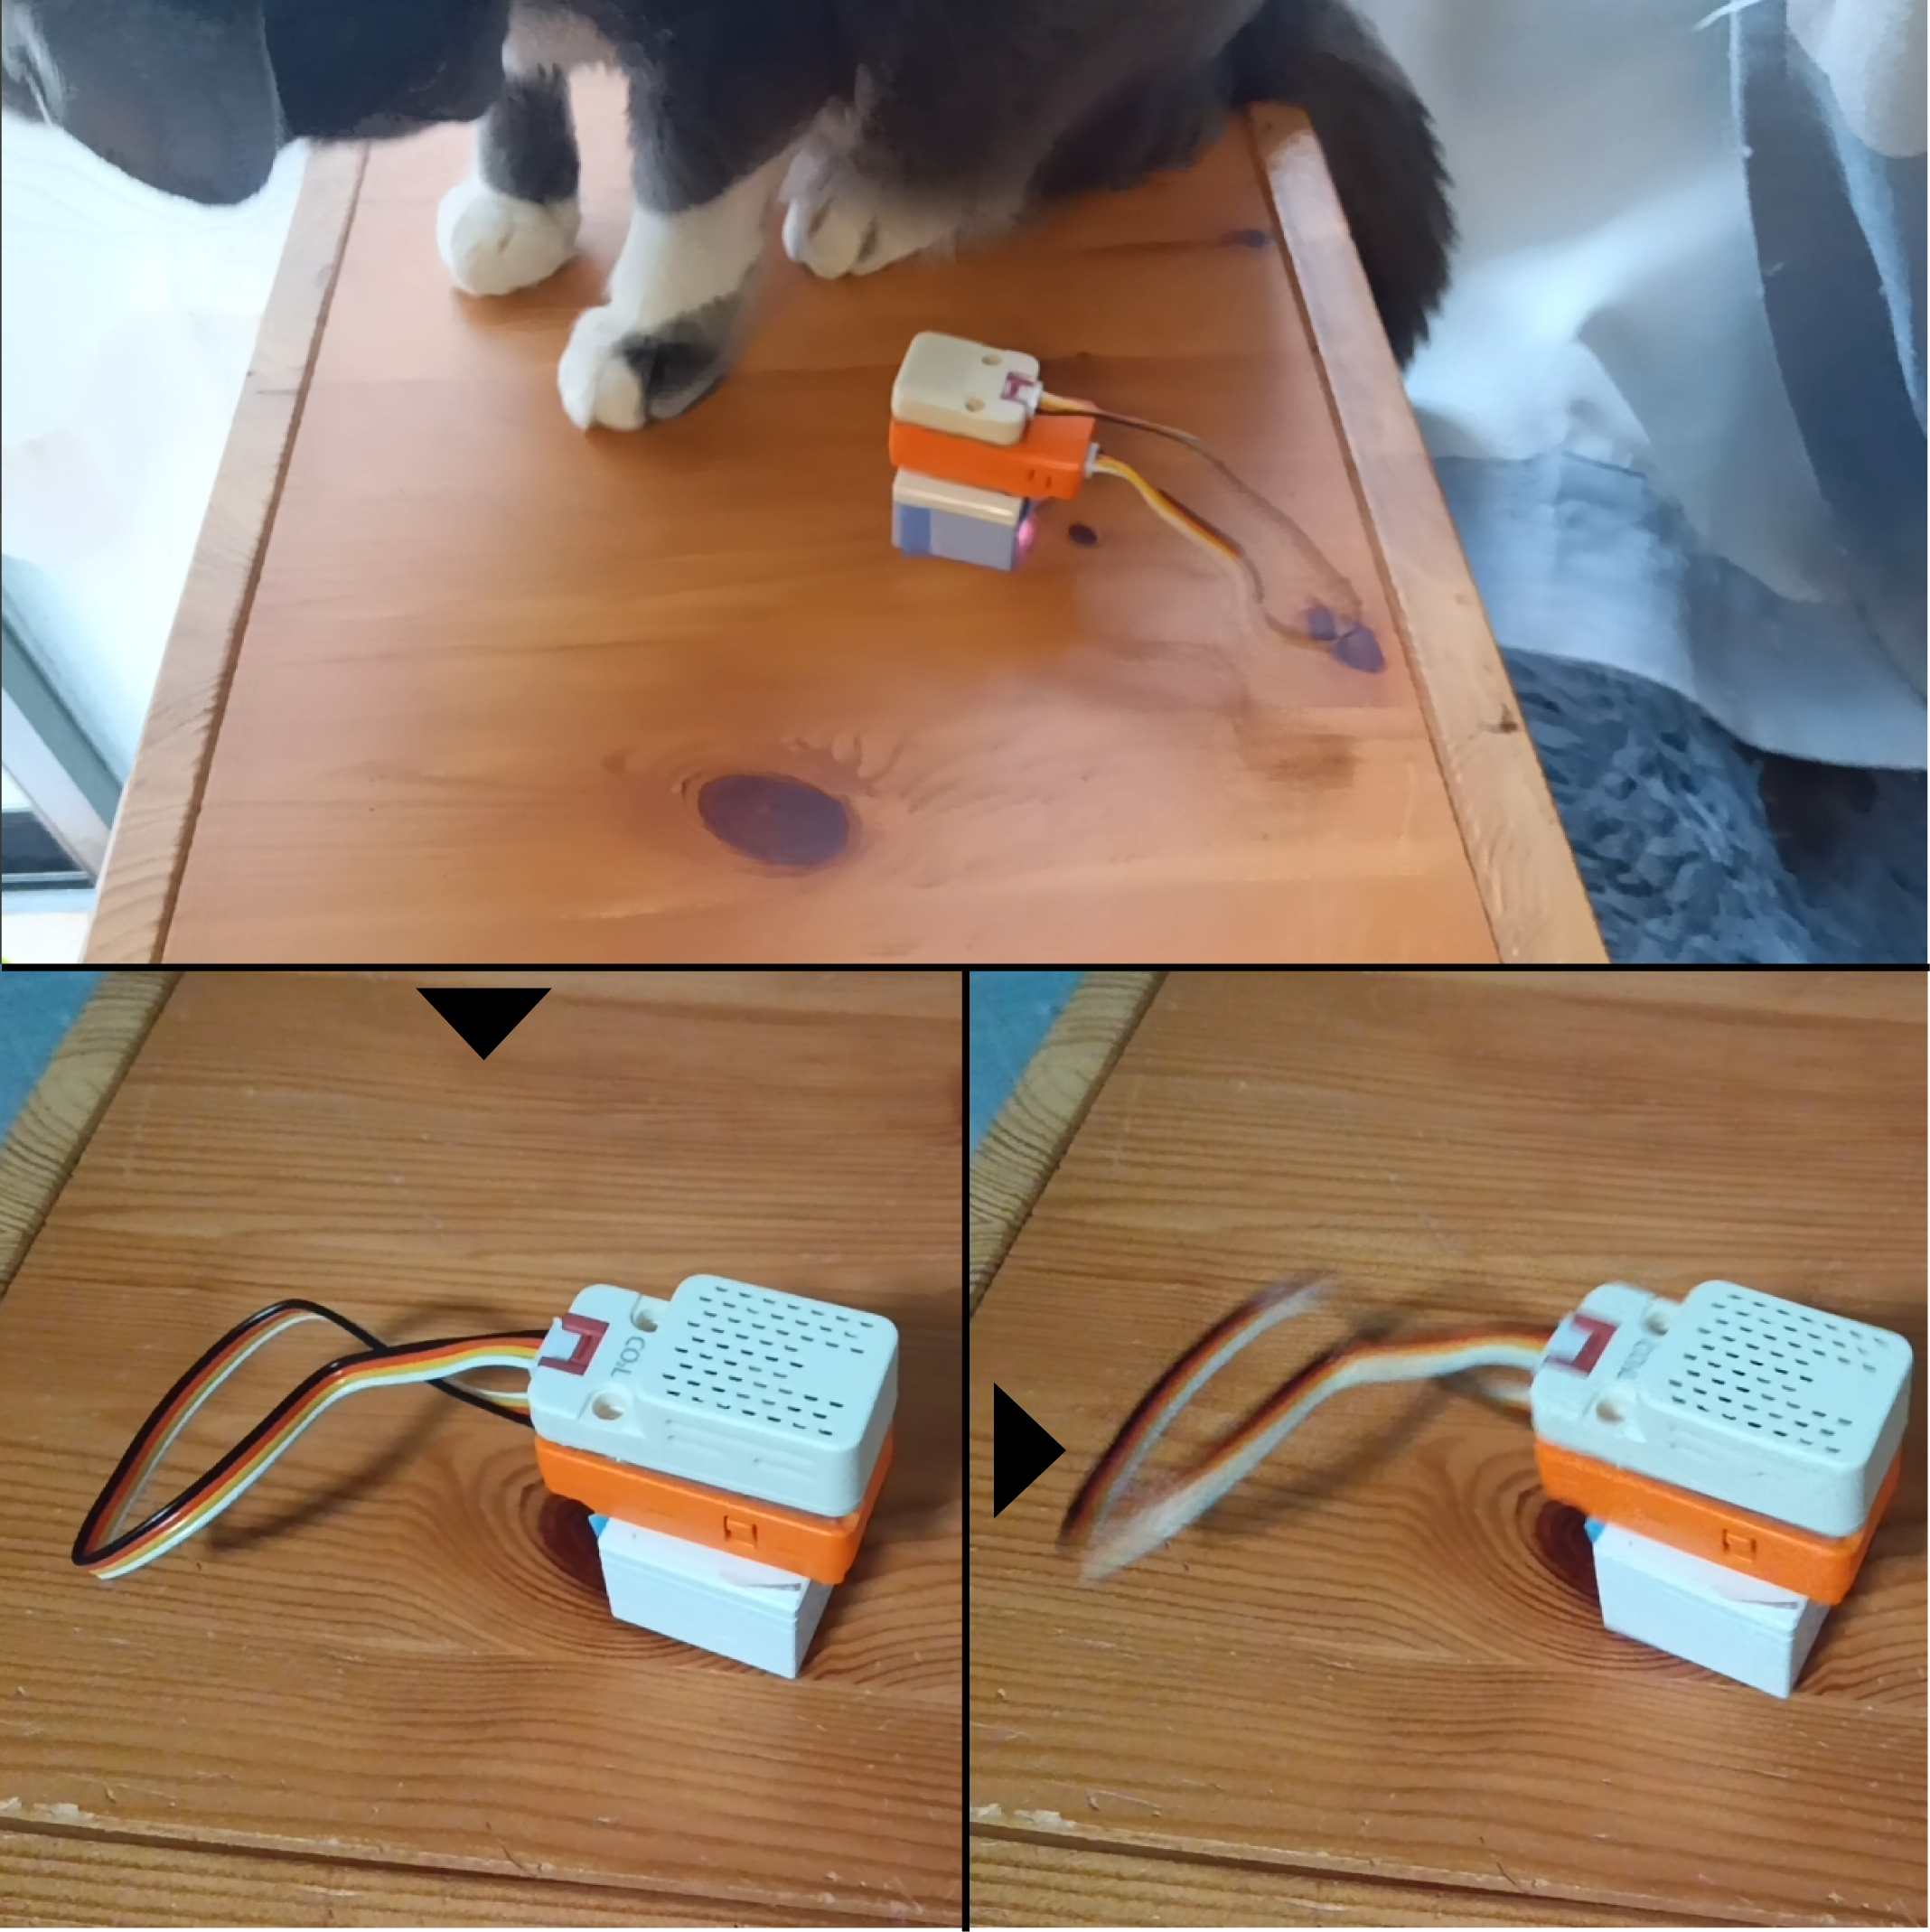
\includegraphics[width=0.22\textwidth]{resources/cat.png} &
    \includegraphics[width=0.22\textwidth]{resources/banana.png} &
    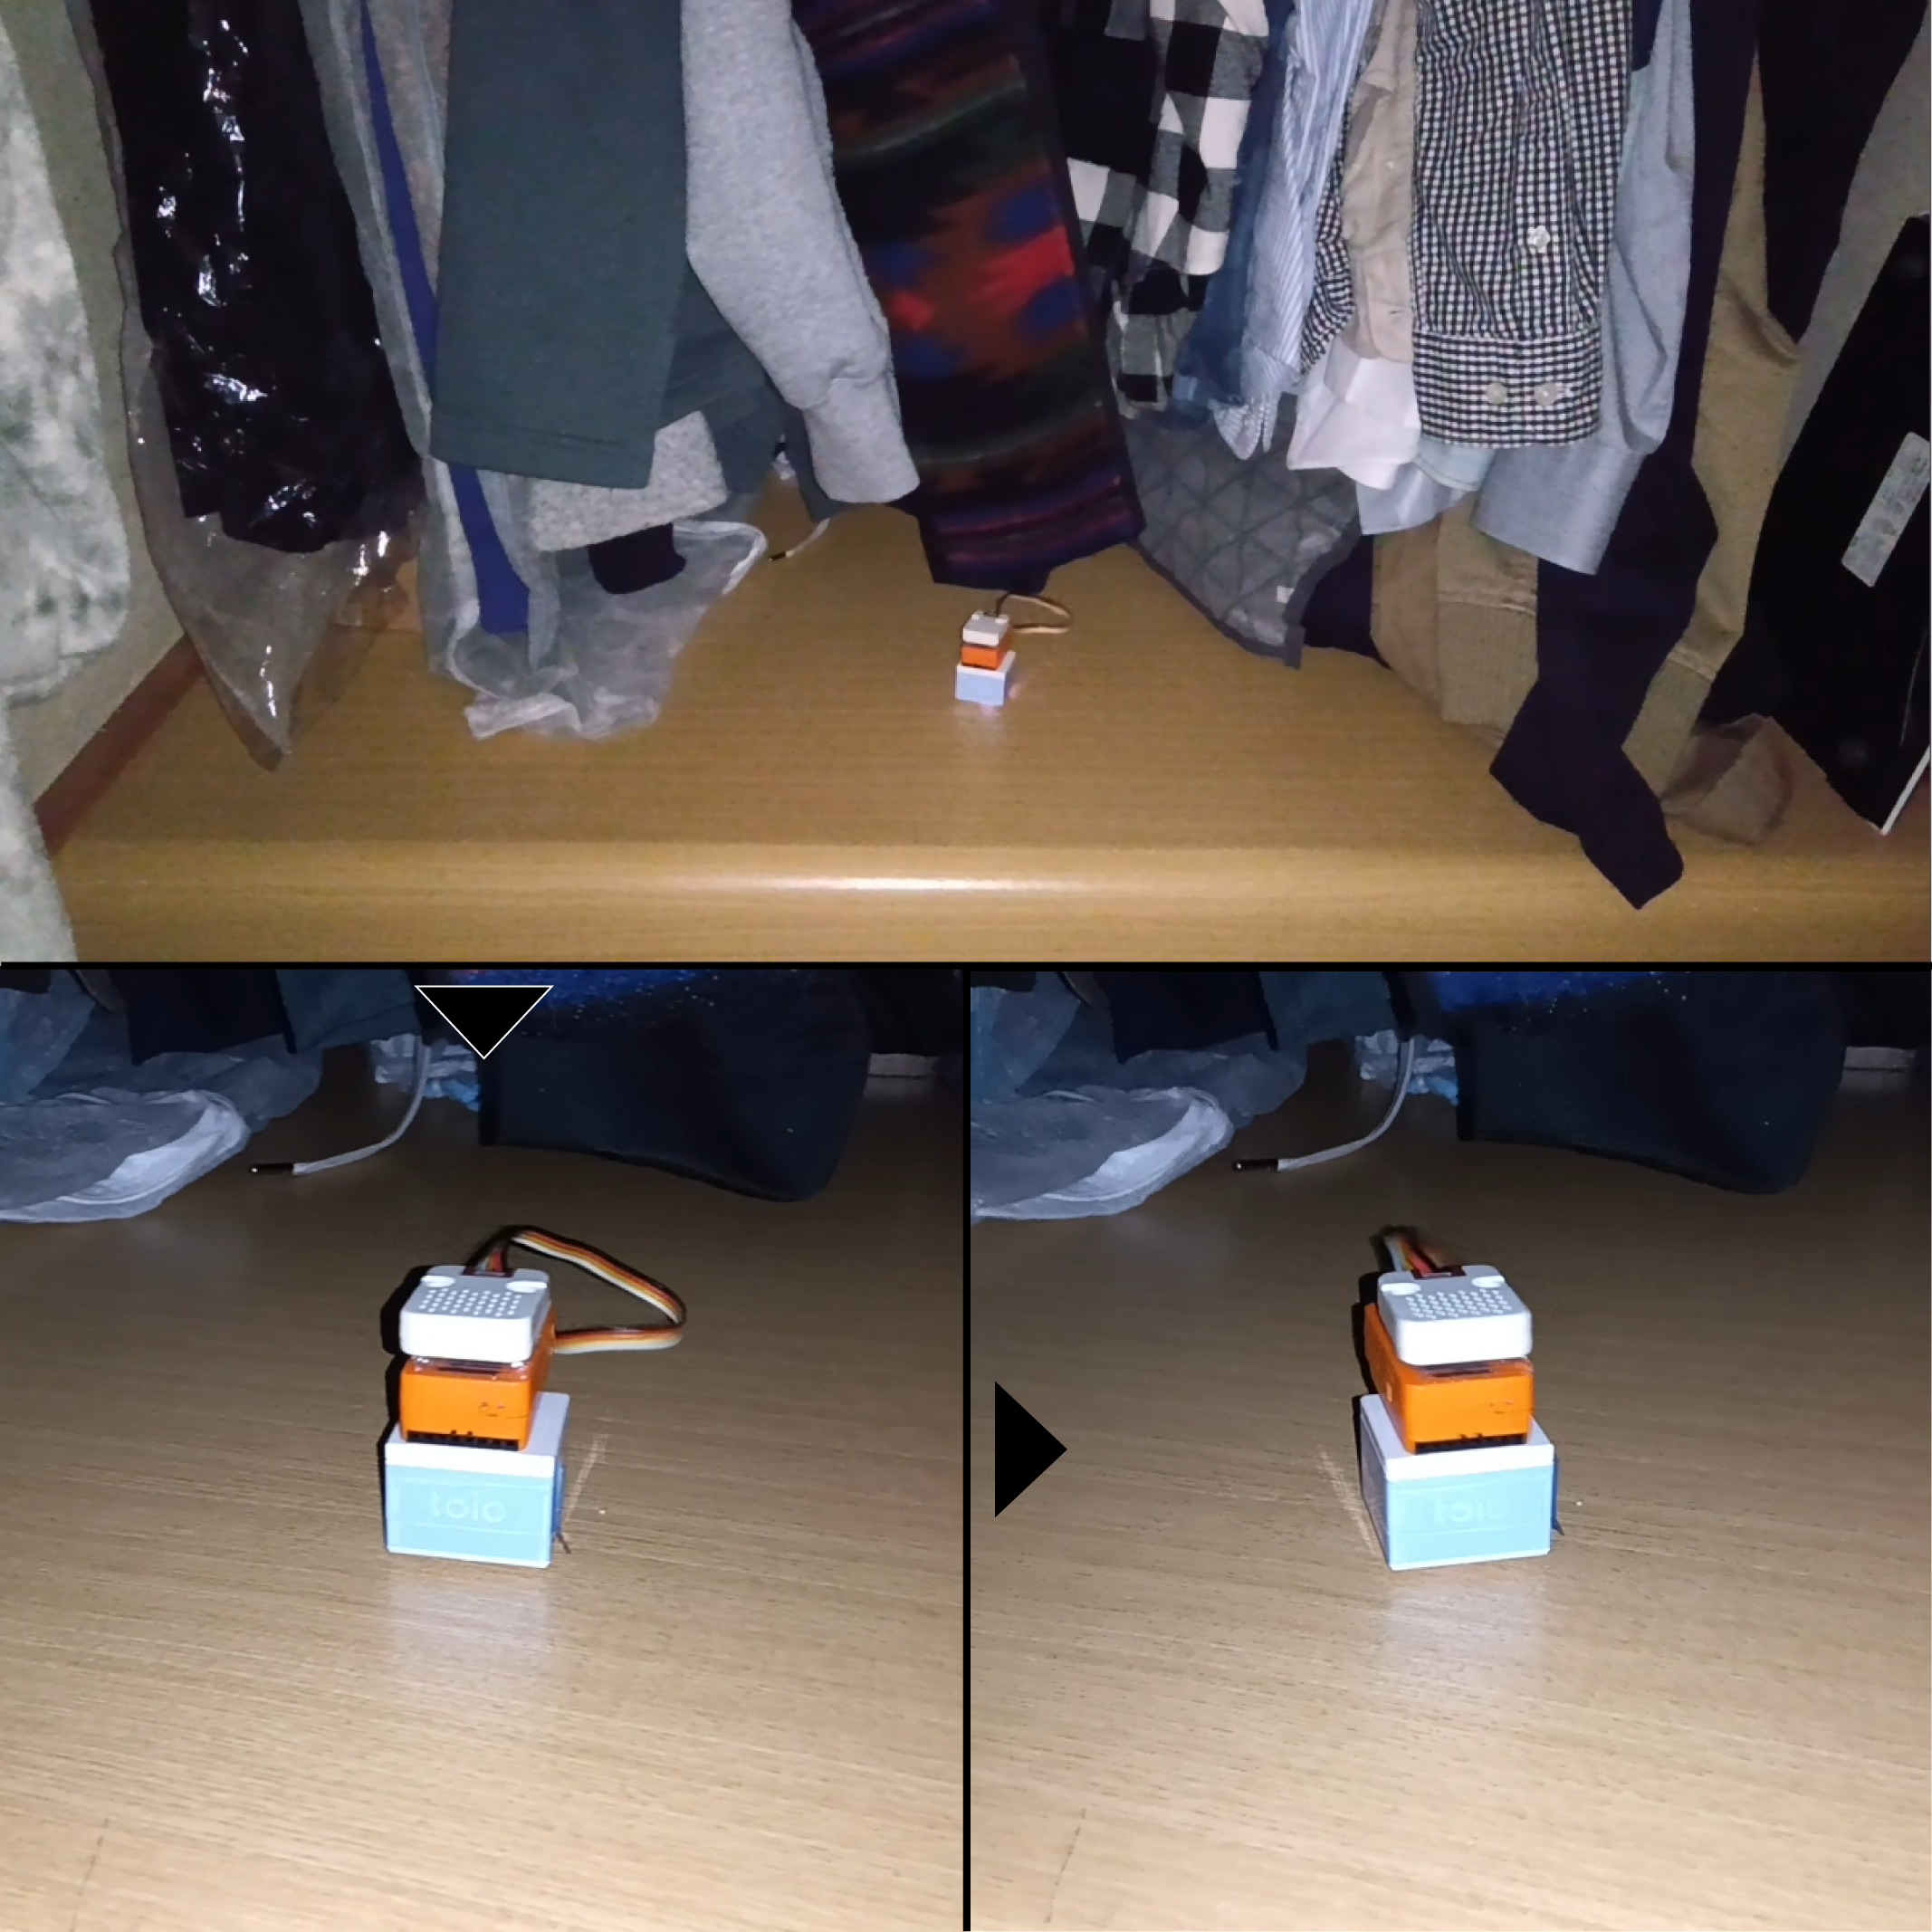
\includegraphics[width=0.22\textwidth]{resources/clothes.png} \\
    人間の気温評価表現 & 猫の気温評価表現 & バナナの保存環境評価表現 & 服の保存環境評価表現
  \end{tabular}
  \caption{システム実装の様子}
  \label{fig:system-test}
\end{figure}

\subsection{他者表現に関する課題}
\begin{enumerate}
  \item \textbf{動作の表現力}:「弱いロボット」のコンセプトを目指したが,実際の動きは機械的で硬い印象となった.フィードバックとして「もっと滑らかな動きが欲しい」との意見があった.

  \item \textbf{他者の識別性}:「動きで伝える」ことを検証するには,外見による先入観を排除する工夫が必要である.

  \item \textbf{通知の適切性}:「快適な環境では警告不要なので動かなくてもよいのでは」という意見もあり,環境状態と動作の対応関係の設計にはさらなる検討が必要である.
\end{enumerate}

\subsection{環境センシングに関する課題}
\begin{enumerate}
  \item \textbf{個人差への対応}:最適な環境の基準には個人差があり,一律の基準では適切な表現ができない可能性がある.
    \begin{itemize}
      \item 対応策:リアルタイムに基準を調整可能なインタフェースの実装
    \end{itemize}

  \item \textbf{空間的整合性}:移動する他者はセンシング位置と他者の位置が一致しない問題がある.
    \begin{itemize}
      \item 対応策:空間的な変化が小さい環境データを中心に評価,または複数センサーの配置
    \end{itemize}

  \item \textbf{時間変化への対応}:時間経過で最適条件が変化する他者は,即時的な評価では表現しきることができない.
    \begin{itemize}
      \item 対応策:環境データの長期記録と分析,それに伴う評価基準の動的調整
    \end{itemize}
\end{enumerate}

\section{技術的課題と限界}
本システムの開発・検証過程で明らかになった技術的課題と限界を以下に整理する.

\begin{enumerate}
  \item \textbf{通信の安定性}:Bluetooth通信に依存しているため,物理的障害物による通信不安定や接続範囲の制限がある.WiFi通信への移行やメッシュネットワークの採用が考えられる.

  \item \textbf{バッテリー持続時間}:M5StickCのバッテリー持続時間は最適化しても数時間程度であり,長期運用には外部電源の検討が必要となる.センサーユニットの動作検証結果を表\ref{table:battery}に示す.

  \item \textbf{衝突と動作空間}:toioの動作には一定の空間が必要であり,狭い場所では衝突によって動けなくなる可能性がある.衝突検知アルゴリズムを実装したが,toio本体に一定以上の速度で衝突が起こらないと反応しない制約がある.

  \item \textbf{動作の硬さ}:「弱いロボット」として自然な「よたよた」とした動きを実現するのは技術的に難しく,細かい動きの組み合わせと調整が必要である.
    \begin{itemize}
      \item toioの動作は基本的に「前進」「回転」「停止」などの離散的なコマンドの組み合わせで構成される
      \item 「よたよた」のような微妙な動きは,これらを細かく組み合わせる必要がある
      \item 不規則性を出しすぎると「よたよた」ではなく病的な動きに見えてしまう可能性
    \end{itemize}

  \item \textbf{外見の識別}:実装したロボットの外見が同一であるため,どの他者を表現しているかの識別が難しい.

  \item \textbf{同時制御数の制限}:現状のシステムアーキテクチャでは同時に制御できるロボットの数に制限があり,多数の他者を同時に表現することは困難である.
\end{enumerate}

\begin{table}[htbp]
  \caption{センサーユニットの動作時間検証結果}
  \label{table:battery}
  \centering
  \begin{tabular}{|l|c|c|c|l|}
    \hline
    センサー構成 & 起動時間 & スリープ時間 & 画面輝度 & 備考 \\
    \hline
    M5StickC+ENV II & 57分 & 10秒 & 1 & 標準設定 \\
    \hline
    M5StickC+ENV II & 86分 & 30秒 & 0 & powerSaveOn関数を使用 \\
    \hline
    M5StickC+CO2L & 38分 & 5秒 & 0 & 標準設定 \\
    \hline
    M5StickC+CO2L & 55分 & 30秒 & 0 & powerSaveOn関数を使用 \\
    \hline
  \end{tabular}
\end{table}

\chapter{結論と展望}

\section{結論}
本研究では,生活環境における他者の環境評価を表現するロボットシステムを提案・実装した.センサーによる環境データの取得,他者基準での評価,ロボットによる動作表現を組み合わせることで,継続的な他者理解の支援を可能とするシステムを構築した.

具体的には,人間,猫,バナナ,衣服といった異なる他者の環境認識を表現するシステムを実装し,それぞれの他者特有の環境評価基準と適切な動作パターンを設計した.これにより,同一のロボットハードウェアで多様な他者の表現を可能にした.人間(気温18-28℃),猫(気温30-38℃),バナナ(気温14-20℃,湿度45-85\%),衣服(湿度65\%以下)といった異なる最適環境条件に基づいて評価を行い,その結果を「弱いロボット」のコンセプトを取り入れた動作で表現することで,ユーザーに自然な気づきを与えることを目指した.

実装の過程では,M5StickCをセンシングユニットとして活用し,toioロボットによる動作表現を実現した.コンポーネント指向アーキテクチャの採用により,システムの拡張性と保守性を確保し,様々な他者パターンの追加を容易にした.

技術的な課題や動作表現の限界は残るものの,本システムは生活環境における他者理解を継続的に支援する新たな手法として,人間と他者の相互理解を促進し,多様な存在が共存する生活空間の実現可能性を示した.

\section{今後の展望}
本研究を通じて明らかになった課題を踏まえ,今後の展開として以下の点について研究を進める.

\subsection{表現力の向上}
\begin{itemize}
  \item \textbf{アクションデザインの改良}
    \begin{itemize}
      \item 「弱いロボット風アクションジェネレーター」の開発
      \item 「よたよた」動作のパラメータ化と細かな調整を可能にするツール
      \item 「弱さ」を表現するための動きパターンライブラリの拡充
    \end{itemize}

  \item \textbf{視覚的識別の改善}
    \begin{itemize}
      \item 同一ハードウェアで異なる他者を識別するための視覚的手がかり
      \item 単純な外装の変更や色による識別など,最小限の変更で認識を助ける工夫
    \end{itemize}

  \item \textbf{ロボット間の協調動作}
    \begin{itemize}
      \item 複数のロボットが連携して一つの他者を表現する手法の開発
      \item 異なる他者間のインタラクション表現
    \end{itemize}
\end{itemize}

\subsection{技術的改善}
\begin{itemize}
  \item \textbf{センシング手法の改善}
    \begin{itemize}
      \item 空間分布を考慮したセンシング手法の開発
      \item 長期的なデータ収集と分析による評価基準の動的調整
      \item バッテリー持続時間の延長(外部電源の活用,消費電力の最適化)
    \end{itemize}

  \item \textbf{通信の安定性向上}
    \begin{itemize}
      \item Bluetooth通信の安定化,またはWiFi通信への移行
      \item メッシュネットワークの採用による広範囲での安定した通信の実現
    \end{itemize}

  \item \textbf{衝突回避アルゴリズムの改良}
    \begin{itemize}
      \item より高精度な障害物検知と回避機能の実装
      \item 生活空間での安定した動作の実現
    \end{itemize}
\end{itemize}

\subsection{応用展開}
\begin{itemize}
  \item \textbf{パーソナライズ機能の実装}
    \begin{itemize}
      \item ユーザー個人の環境評価基準を学習し,適応するシステムの開発
      \item リアルタイムに基準を調整可能なインタフェースの実装
    \end{itemize}

  \item \textbf{情報システムとの連携}
    \begin{itemize}
      \item システム状態やイベントの通知手段としての活用
      \item デジタルネイチャーの文脈における他者概念の拡張
      \item 情報環世界と物理環世界の橋渡し役としての機能
    \end{itemize}

  \item \textbf{異なるハードウェアによる新たな体験の創出}
    \begin{itemize}
      \item より表現力の高いロボットプラットフォームへの応用
      \item キャラクター化による親しみやすさの向上
    \end{itemize}
\end{itemize}

\subsection{具体的なユースケース}
本システムは以下のような具体的なユースケースでの活用が考えられる:

\begin{enumerate}
  \item \textbf{介護シーン}:介護者が作業中でも,高齢者の部屋の環境を監視し,必要に応じて介護者に通知するエージェントとして機能する.通知は機械的なアラートではなく,ロボットの「よたよた」とした動きで自然な気づきを促す.

  \item \textbf{遠隔ワーク環境}:在宅勤務中,子供部屋など別の部屋の環境を監視し,異常があれば作業中の親に通知する.

  \item \textbf{植物ケア}:植物の視点から見た適切な環境(光,温度,湿度,CO2濃度など)を表現し,人間に世話を促す.

  \item \textbf{食品保存}:冷蔵庫や保存庫内の食品の視点から,適切な保存環境を表現する.例えばバナナなど特定の食品に適した温度・湿度条件を他者として表現する.
\end{enumerate}

これらのユースケースは,従来の機械的なセンサー通知システムとは異なり,他者の視点を通じた感覚的な理解を促進する.本研究で提案したシステムは,生活空間における多様な存在との共生を支援する新たなインタラクションの可能性を示すものである.

\chapteraddtoc{謝辞}
本稿の執筆および研究にあたって,ご指導いただいた佐藤弘樹先生に深く感謝いたします.

\vspace{3\zh}
\begin{flushright}
  2025年3月19日 \\
  宮城大学 事業構想学群 価値創造デザイン学類 \\
  感性情報デザインコース \\
  中村龍造
\end{flushright}

\newpage
\renewcommand{\refname}{\huge 参考文献}
\bibliographystyle{junsrt}
\bibliography{ref}
\addcontentsline{toc}{chapter}{参考文献}

\end{document}
